\documentclass[12pt]{article}
\usepackage[margin=1in]{geometry}
\usepackage{graphicx}
\usepackage{amsmath}
\usepackage{tikz}
\usepackage{hyperref}
\usepackage{enumitem}

\newcommand{\f}[1]{o_{#1}x_{#1}y_{#1}z_{#1}}
\newcommand{\fromslides}{{\\ \color{blue} \hspace*{\fill}(from lecture slides)} \\}
\newcommand{\bydefn}{{\\ \color{blue} \hspace*{\fill}(by definition)} \\}
\newcommand{\given}{{\\ \color{blue} \hspace*{\fill}(given)} \\}

\newcommand{\rx}[1]{\begin{bmatrix} 1 & 0 & 0 \\ 0 & cos(#1) & -sin(#1) \\ 0 & sin(#1) & cos(#1) \end{bmatrix}}
\newcommand{\ry}[1]{\begin{bmatrix} cos(#1) & 0 & sin(#1) \\ 0 & 1 & 0 \\ -sin(#1) & 0 & cos(#1) \end{bmatrix}}
\newcommand{\rz}[1]{\begin{bmatrix} cos(#1) & -sin(#1) & 0 \\ sin(#1) & cos(#1) & 0 \\ 0 & 0 & 1 \end{bmatrix}}

\title{CSci 5551 - HW1}
\author{Yashasvi Sriram Patkuri\\patku001@umn.edu}

\begin{document}
\maketitle
\pagebreak

%--------------------------------------------------------------------------------
\section{}
Let $ \f{\frac{1}{2}} $ represent the coordinate system formed by rotating $ \f{0} $ by $ \frac{\pi}{2} $ radians about the x-axis.
Let this rotation be denoted by $ R_1 $. Using basic matrices
\begin{equation}
  R_1 \equiv \rx{\frac{\pi}{2}} \equiv \begin{bmatrix} 1 & 0 & 0 \\ 0 & 0 & -1 \\ 0 & 1 & 0 \end{bmatrix}
\end{equation}
\fromslides

$ \f{1} $ represents the coordinate system formed by rotating $ \f{\frac{1}{2}} $ by$ \frac{\pi}{2} $ radians about the fixed frame Y-axis.
Let this rotation be denoted by $ R_2 $. Using basic matrices
\begin{equation}
  R_2 \equiv \ry{\frac{\pi}{2}} \equiv \begin{bmatrix} 0 & 0 & 1 \\ 0 & 1 & 0 \\ -1 & 0 & 0 \end{bmatrix}
\end{equation}
\fromslides

For two consecutive fixed frame rotations denoted by $ R_1, R_2 $ rotation matrices, the composite rotation matrix, say R $ \equiv $ $ R_2 * R_1 $

\begin{equation}
  R
  \equiv R_2 * R_1
  \equiv \begin{bmatrix} 0 & 0 & 1 \\ 0 & 1 & 0 \\ -1 & 0 & 0 \end{bmatrix} * \begin{bmatrix} 1 & 0 & 0 \\ 0 & 0 & -1 \\ 0 & 1 & 0 \end{bmatrix}
  \equiv \begin{bmatrix} 0 & 1 & 0 \\ 0 & 0 & -1 \\ -1 & 0 & 0 \end{bmatrix}
\end{equation}
\fromslides


The sketches of frames $ \f{1} $, $ \f{\frac{1}{2}} $ and $ \f{1} $ are drawn in figure \ref{fig:q1}.

\begin{figure}[htpb]
  \centering
  \begin{tikzpicture}[x=1cm, y=1cm, z=-0.6cm]
      \draw [->] (0,0,0) -- (4,0,0) node [right] {$x_0$};
      \draw [->] (0,0,0) -- (0,4,0) node [left] {$y_0$};
      \draw [->] (0,0,0) -- (0,0,4) node [left] {$z_0$};
  \end{tikzpicture}

  \begin{tikzpicture}[x=1cm, y=1cm, z=-0.6cm]
      \draw [->] (0,0,0) -- (4,0,0) node [right] {$x_{\frac{1}{2}}$};
      \draw [->] (0,0,0) -- (0,0,4) node [left] {$y_{\frac{1}{2}}$};
      \draw [->] (0,0,0) -- (0,-4,0) node [left] {$z_{\frac{1}{2}}$};
  \end{tikzpicture}

  \begin{tikzpicture}[x=1cm, y=1cm, z=-0.6cm]
      \draw [->] (0,0,0) -- (0,0,-4) node [left] {$x_1$};
      \draw [->] (0,0,0) -- (4,0,0) node [right] {$y_1$};
      \draw [->] (0,0,0) -- (0,-4,0) node [left] {$z_1$};
  \end{tikzpicture}
\caption{Rotations by $ \frac{\pi}{2} $ radians about fixed X and Y axes consecutively}
  \label{fig:q1}
\end{figure}

\pagebreak

%--------------------------------------------------------------------------------
\section{}

Given
\begin{equation}
  R_{12} \equiv \begin{bmatrix} 1 & 0 & 0 \\ 0 & \frac{1}{2} & -\frac{\sqrt{3}}{2} \\ 0 & \frac{\sqrt{3}}{2} & \frac{1}{2} \end{bmatrix}
\end{equation}
\begin{equation}
  R_{13} \equiv \begin{bmatrix} 0 & 0 & -1 \\ 0 & 1 & 0 \\ 1 & 0 & 0 \end{bmatrix}
\end{equation}

For any physical vector p, let $ p^{i} $ be its representation in ith coordinate system
\begin{equation}
  \label{eq:21}
  p^{2} \equiv R_{21} * p^{1}
\end{equation}
\begin{equation}
  \label{eq:22}
  p^{1} \equiv R_{13} * p^{3}
\end{equation}
\bydefn

Identities \ref{eq:21} and \ref{eq:22} imply
\begin{equation}
  \label{eq:23}
  p^{2} \equiv R_{21} * R_{13} * p^{3}
\end{equation}

But
\begin{equation}
  \label{eq:24}
  p^{2} \equiv R_{23} * p^{3}
\end{equation}
\bydefn

From identities \ref{eq:23} and \ref{eq:24}
\begin{equation}
  \label{eq:25}
  R_{23} \equiv R_{21} * R_{13}
\end{equation}

But
\begin{equation}
  \label{eq:26}
  R_{21} \equiv R_{12}^{T}
\end{equation}
\fromslides

Identities \ref{eq:25} and \ref{eq:26} imply
\begin{equation}
  \label{eq:27}
  R_{23} \equiv R_{12}^T * R_{13}
  \equiv \begin{bmatrix} 1 & 0 & 0 \\ 0 & \frac{1}{2} & \frac{\sqrt{3}}{2} \\ 0 & -\frac{\sqrt{3}}{2} & \frac{1}{2} \end{bmatrix} * \begin{bmatrix} 0 & 0 & -1 \\ 0 & 1 & 0 \\ 1 & 0 & 0 \end{bmatrix}
  \equiv \begin{bmatrix} 0 & 0 & -1 \\ \frac{\sqrt{3}}{2} & \frac{1}{2} & 0 \\ \frac{1}{2} & -\frac{\sqrt{3}}{2} & 0 \end{bmatrix}
\end{equation}

\pagebreak

%--------------------------------------------------------------------------------
\section{}

Let us represent the Z-X-Z angles by $ \theta_1, \theta_2, \theta_3 $ instead of $ \phi, \theta, \psi $ respectively for simplicity.

First we build rotation matrix corresponding to each Eular angle.
Using basic rotation matrices we get
\begin{equation}
  \label{eq:31}
  R_{\theta_1,z} \equiv \rz{\theta_1}
\end{equation}
\begin{equation}
  \label{eq:32}
  R_{\theta_2,x} \equiv \rx{\theta_2}
\end{equation}
\begin{equation}
  \label{eq:33}
  R_{\theta_3,z} \equiv \rz{\theta_3}
\end{equation}

Eular angles correspond to consecutive current frame rotations.
For consecutive current frame rotations $ R_1, R_2, R_3 $, the composite rotation matrix is say R is given by
\begin{equation}
  \label{eq:34}
  R \equiv R_1 * R_2 * R_3
\end{equation}
\fromslides

Substituting equations \ref{eq:31}, \ref{eq:32}, \ref{eq:33} in \ref{eq:34} we get,
\begin{equation}
  \label{eq:35}
  R_{ZXZ} \equiv R_{\theta_1,z} * R_{\theta_2,x} * R_{\theta_3,z}
\end{equation}
where $ R_{ZXZ} $ represents rotation matrix corresponding to the set of Z-X-Z eular angles.

\[
  R_{ZXZ} \equiv \rz{\theta_1} * \rx{\theta_2} * \rz{\theta_3}
\]
\[
  R_{ZXZ} \equiv \begin{bmatrix} c1 & -s1.c2 & s1.s2 \\ s1 & c1.c2 & -c1.s2 \\ 0 & s2 & c2 \end{bmatrix} * \rz{\theta_3}
\]
Where ci represents $ cos(\theta_i) $ and si represents $ sin(\theta_i) $
\begin{equation}
  \label{eq:36}
  R_{ZXZ} \equiv \begin{bmatrix} c1.c3 - s1.c2.s3 & -c1.s3 - s1.c2.c3 & s1.s2 \\ s1.c3 + c1.c2.s3 & -s1.s3 + c1.c2.c3 & -c1.s2 \\ s2.s3 & s2.c3 & c2 \end{bmatrix}
\end{equation}

Equation \ref{eq:36} is the rotation matrix corresponding to Z-X-Z Eular angles.

\subsection{$sin(\theta) = 0$}
For us $\theta_2$ represents $\theta$.
$sin(\theta_2) = 0$ implies $cos(\theta_2) = 1$. Substituting these in equation \ref{eq:36} we get
\begin{equation}
  \label{eq:37}
  R_{ZXZ} \equiv \begin{bmatrix} c1.c3 - s1.s3 & -c1.s3 - s1.c3 & 0 \\ s1.c3 + c1.s3 & -s1.s3 + c1.c3 & 0 \\ 0 & 0 & 1 \end{bmatrix}
\end{equation}
But
\begin{equation}
  \label{eq:38}
  sin(a + b) = sin(a)cos(b) + cos(a)sin(b)
\end{equation}
\begin{equation}
  \label{eq:39}
  cos(a + b) = cos(a)cos(b) - sin(a)sin(b)
\end{equation}

From equations \ref{eq:37}, \ref{eq:38} and \ref{eq:39} we can write
\begin{equation}
  \label{eq:310}
  R_{ZXZ} \equiv \rz{\theta_1 + \theta_3}
\end{equation}
Therefore, when $sin(\theta) = 0$ the composite rotation matrix is identical to rotation about Z-axis by $ \theta_1 + \theta_3 $.
{\color{red} Does it lose a degree of freedom? Gimbal lock?}.

\pagebreak

%--------------------------------------------------------------------------------
\section{}
\subsection{}
The general form of a transformation matrix is
\[
  H_{y}^{x} \equiv \begin{bmatrix} R_{y}^{x} & p_{y}^{x} \\ O_{1x3} & 1 \end{bmatrix}
\]
Where
\begin{enumerate}[nolistsep]
  \item $ R_{y}^{x} $ represents rotation matrix of coordinate system y w.r.t coordinate system x
  \item $ p_{y}^{x} $ represents position vector of origin of coordinate system y in coordinate system x
  \item $ O_{1x3} $ represents a 1x3 zero matrix
\end{enumerate}
\bydefn

As there is no rotation b/w coordinate systems 1 and 0 and 2 and 0, the rotation matrices $ R_{1}^{0}, R_{2}^{0} \equiv I_{3x3} $ where $ I_{3x3} $ represents identity matrix of order 3. Therefore to calculate $ H_{1}^{0}, H_{2}^{0} $ we only need $ p_{1}^{0}, p_{2}^{0} $.

\begin{figure}[h]
  \centering
  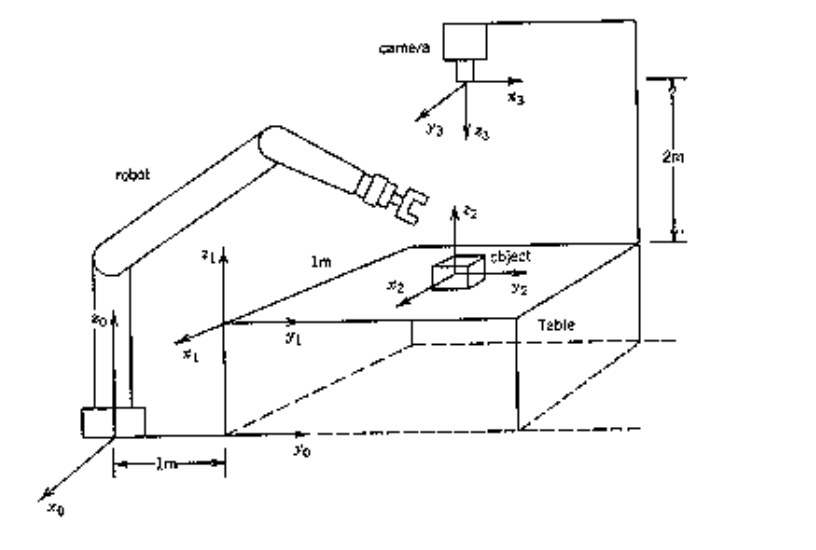
\includegraphics[width=0.8\textwidth]{p4-fig.png}
  \caption{Arrangement of coordinate systems 0, 1, 2, 3}
  \label{fig:p4}
\end{figure}

In coordinate system 0, the origin $ p_{1} $ of coordinate system 1 has
\begin{enumerate}[nolistsep]
  \item x-coordinate = 0, because it is in YZ plane (assumed from figure \ref{fig:p4})
  \item y-coordinate = 1, because it lies on nearest leg of the table which is 1m far from the origin of 0 in y direction.
  \item z-coordinate = 1, because it lies on table top which is 1m far from the origin of 0 in the z direction.
\end{enumerate}
Therefore
\[
  p_{1}^{0} \equiv \begin{bmatrix} 0 \\ 1 \\ 1 \end{bmatrix}
\]
Which implies
\[
  H_{1}^{0}
  \equiv \begin{bmatrix} I_{3x3} & \begin{bmatrix} 0 \\ 1 \\ 1 \end{bmatrix} \\ O_{1x3} & 1 \end{bmatrix}
  \equiv \begin{bmatrix}
          1 & 0 & 0 & 0\\
          0 & 1 & 0 & 1\\
          0 & 0 & 1 & 1\\
          0 & 0 & 0 & 1
        \end{bmatrix}
\]

In coordinate system 0, the origin $ p_{2} $ of coordinate system 2 has
\begin{enumerate}[nolistsep]
  \item x-coordinate = -0.5, because it is at the center of cube which is at the center of table top. Distance from origin of 0 to center of table to is 0.5m in the opposite direction of x-axis and hence the coordinate value.
  \item y-coordinate = 1.5, because it is at the center of cube which is at the center of table top. Distance from origin of 0 to center of table to is 1.5m in the direction of y-axis and hence the coordinate value.
  \item z-coordinate = 1.1, because it is at the center of cube which is at the center of table top. Distance from origin of 0 to table top in z-direction is 1m. But the origin of 2 is at center of cube of width 0.2m. This adds a (0.2 / 2)m height and hence the coordinate value 1 + 0.1 = 1.1
\end{enumerate}
Therefore
\[
  p_{2}^{0} \equiv \begin{bmatrix} -0.5 \\ 1.5 \\ 1.1 \end{bmatrix}
\]
Which implies
\[
  H_{2}^{0}
  \equiv \begin{bmatrix} I_{3x3} & \begin{bmatrix} -0.5 \\ 1.5 \\ 1.1 \end{bmatrix} \\ O_{1x3} & 1 \end{bmatrix}
  \equiv \begin{bmatrix}
          1 & 0 & 0 & -0.5\\
          0 & 1 & 0 & 1.5\\
          0 & 0 & 1 & 1.1\\
          0 & 0 & 0 & 1
        \end{bmatrix}
\]

In coordinate system 0, the origin $ p_{3} $ of coordinate system 3 has same x and y coordinates as $ p_{2}^{0} $ because the camera (the coordinate system 3 attached to it) is situated directly above center of cube 2m from table top.
\given
\begin{enumerate}[nolistsep]
  \item x-coordinate = -0.5
  \item y-coordinate = 1.5
  \item z-coordinate = 3, because it is 2m above the table top i.e. 1+2m above the ground
\end{enumerate}
Therefore
\[
  p_{1}^{0} \equiv \begin{bmatrix} -0.5 \\ 1.5 \\ 3 \end{bmatrix}
\]
Coordinate system 3 is rotated w.r.t coordinate system 0, therefore $ R_{3}^{0} \not\equiv I_{3x3} $.
\[
  R_{3}^{0}
  \equiv \begin{bmatrix}
        i_3.i_0 & j_3.i_0 & k_3.i_0\\
        i_3.j_0 & j_3.j_0 & k_3.j_0\\
        i_3.k_0 & j_3.k_0 & k_3.k_0\\
        \end{bmatrix}
  \equiv \begin{bmatrix}
        0 & 1 & 0\\
        1 & 0 & 0\\
        0 & 0 & -1\\
        \end{bmatrix}
\]
\fromslides

Which implies
\[
  H_{3}^{0}
  \equiv \begin{bmatrix} I_{3x3} & \begin{bmatrix} 0 \\ 1 \\ 1 \end{bmatrix} \\ O_{1x3} & 1 \end{bmatrix}
  \equiv \begin{bmatrix}
          0 & 1 & 0 & -0.5\\
          1 & 0 & 0 & 1.5\\
          0 & 0 & -1 & 3\\
          0 & 0 & 0 & 1
        \end{bmatrix}
\]

\subsection{}
{\color{red} Does inverse of homogeneous transformation always exist?}

For any physical vector v,
\[
  v^{0} \equiv H_{2}^{0} * v^{2}
\]
\bydefn
Multiplying by $ H_{2}^{0}^{-1} $ on both sides from right hand.
\[
  H_{2}^{0}^{-1} * v^{0} \equiv H_{2}^{0}^{-1} * H_{2}^{0} * v^{2}
\]
\[
  H_{2}^{0}^{-1} * v^{0} \equiv v^{2}
\]
\[
  v^{2} \equiv H_{2}^{0}^{-1} * v^{0}
\]

But also
\[
  v^{2} \equiv H_{0}^{2} * v^{0}
\]
\bydefn
Therefore
\[
  H_{0}^{2} \equiv H_{2}^{0}^{-1}
  \equiv \begin{bmatrix}
          1 & 0 & 0 & -0.5\\
          0 & 1 & 0 & 1.5\\
          0 & 0 & 1 & 1.1\\
          0 & 0 & 0 & 1
        \end{bmatrix}^{-1}
  \equiv \begin{bmatrix}
          1 & 0 & 0 & 0.5\\
          0 & 1 & 0 & -1.5\\
          0 & 0 & 1 & -1.1\\
          0 & 0 & 0 & 1
        \end{bmatrix}
\]
But
\[
  v^{0} \equiv H_{3}^{0} * v^{3}
\]
\[
  v^{2} \equiv H_{0}^{2} * v^{0}
\]
\bydefn

Therefore combining above two equations
\[
  v^{2} \equiv H_{0}^{2} * H_{3}^{0} * v^{3}
\]
But
\[
  V^{2} \equiv H_{3}^{2} * v^{3}
\]
\bydefn

Therefore
\[
  H_{3}^{2} \equiv H_{0}^{2} * H_{3}^{0}
  \equiv \begin{bmatrix}
          1 & 0 & 0 & 0.5\\
          0 & 1 & 0 & -1.5\\
          0 & 0 & 1 & -1.1\\
          0 & 0 & 0 & 1
        \end{bmatrix}
        * \begin{bmatrix}
          0 & 1 & 0 & -0.5\\
          1 & 0 & 0 & 1.5\\
          0 & 0 & -1 & 3\\
          0 & 0 & 0 & 1
        \end{bmatrix}
  \equiv \begin{bmatrix}
          0 & 1 & 0 & 0\\
          1 & 0 & 0 & 0\\
          0 & 0 & -1 & 1.9\\
          0 & 0 & 0 & 1
        \end{bmatrix}
\]

\end{document}
